\section{Arduino}
Arduino merupakan perangkat keras berupa papan mikrokontroler yang bersifat \textit{Open Source} sehingga bisa dibuat oleh siapa saja. 
Jenis dari kartu arduino sendiri terdiri dari beberapa macam seperti :
\begin{itemize}
\item Arduino Uno 
\item Arduino Diecimila
\item Arduino Duemilanove
\item Arduino Leonardo
\item Arduino Mega
\item Arduino Nano
\end{itemize}
Meskipun memiliki jenis yang berbeda-beda, namun prinsip yang digunakan dalam pemograman yang diperlukan hampir sama atau menyerupai. Yang membedakan dari jenis-jenis arduino diatas adalah kelengkapan peralatan atau fasilitas dan pin-pin yang perlu digunakan. 

Arduino sendiri dibuat dengan tujuan untuk memudahkan dalam melakukan eksperimen atau perwujudan berbagai percobaan yang menggunakan peralatan berbasis mikrokontroler seperti :
\begin{itemize}
\item Pendeteksi bencana alam
\item Pelacakan lokasi kendaraan
\item Penyiraman tanaman secara otomatis
\item Sistem Lock Door pada sebuah ruangan
\item Sistem pendeteksi terhadap manusia
\end{itemize}
\subsection{Arduino Uno}
Arduino Uno merupakan salah satu jenis dari berbagai macam jenis kartu Arduino. Memiliki ukuran sebesar kartu kredit, papan kecil tersebut mengandung mikro kontroler dan sejumlah I/0 (\textit{Input / Output}) yang dapat memudahkan pengguna agar dapat melakukan berbagai eksperimen ataupun project elektronika yang dikhususkan untuk tujuan tertentu.

Untuk spesifikasi Arduino Uno sendiri dilengkapi dengan :
\begin{enumerate}
\item SRAM (\textit{Static Random-Acces Memory}) berukuran 2 KB, fungsinya adalah untuk menampung data atau hasil pemrosesan data selama Arduino menerima pasokan catu daya.
\item \textit{Flash Memory} berukuran 32 KB, fungsinya untuk menaruh program yang telah kita buat.
\item EEPROM  (\textit{Erasable Programmable Read-Only Memory}), fungsinya untuk menaruh program bawaan dari arduino Uno dan sebagian lagi dapat kita manfaatkan untuk menaruh data milik kita sendiri secara permanen
\end{enumerate}

\begin{figure}[!htbp]
\centering
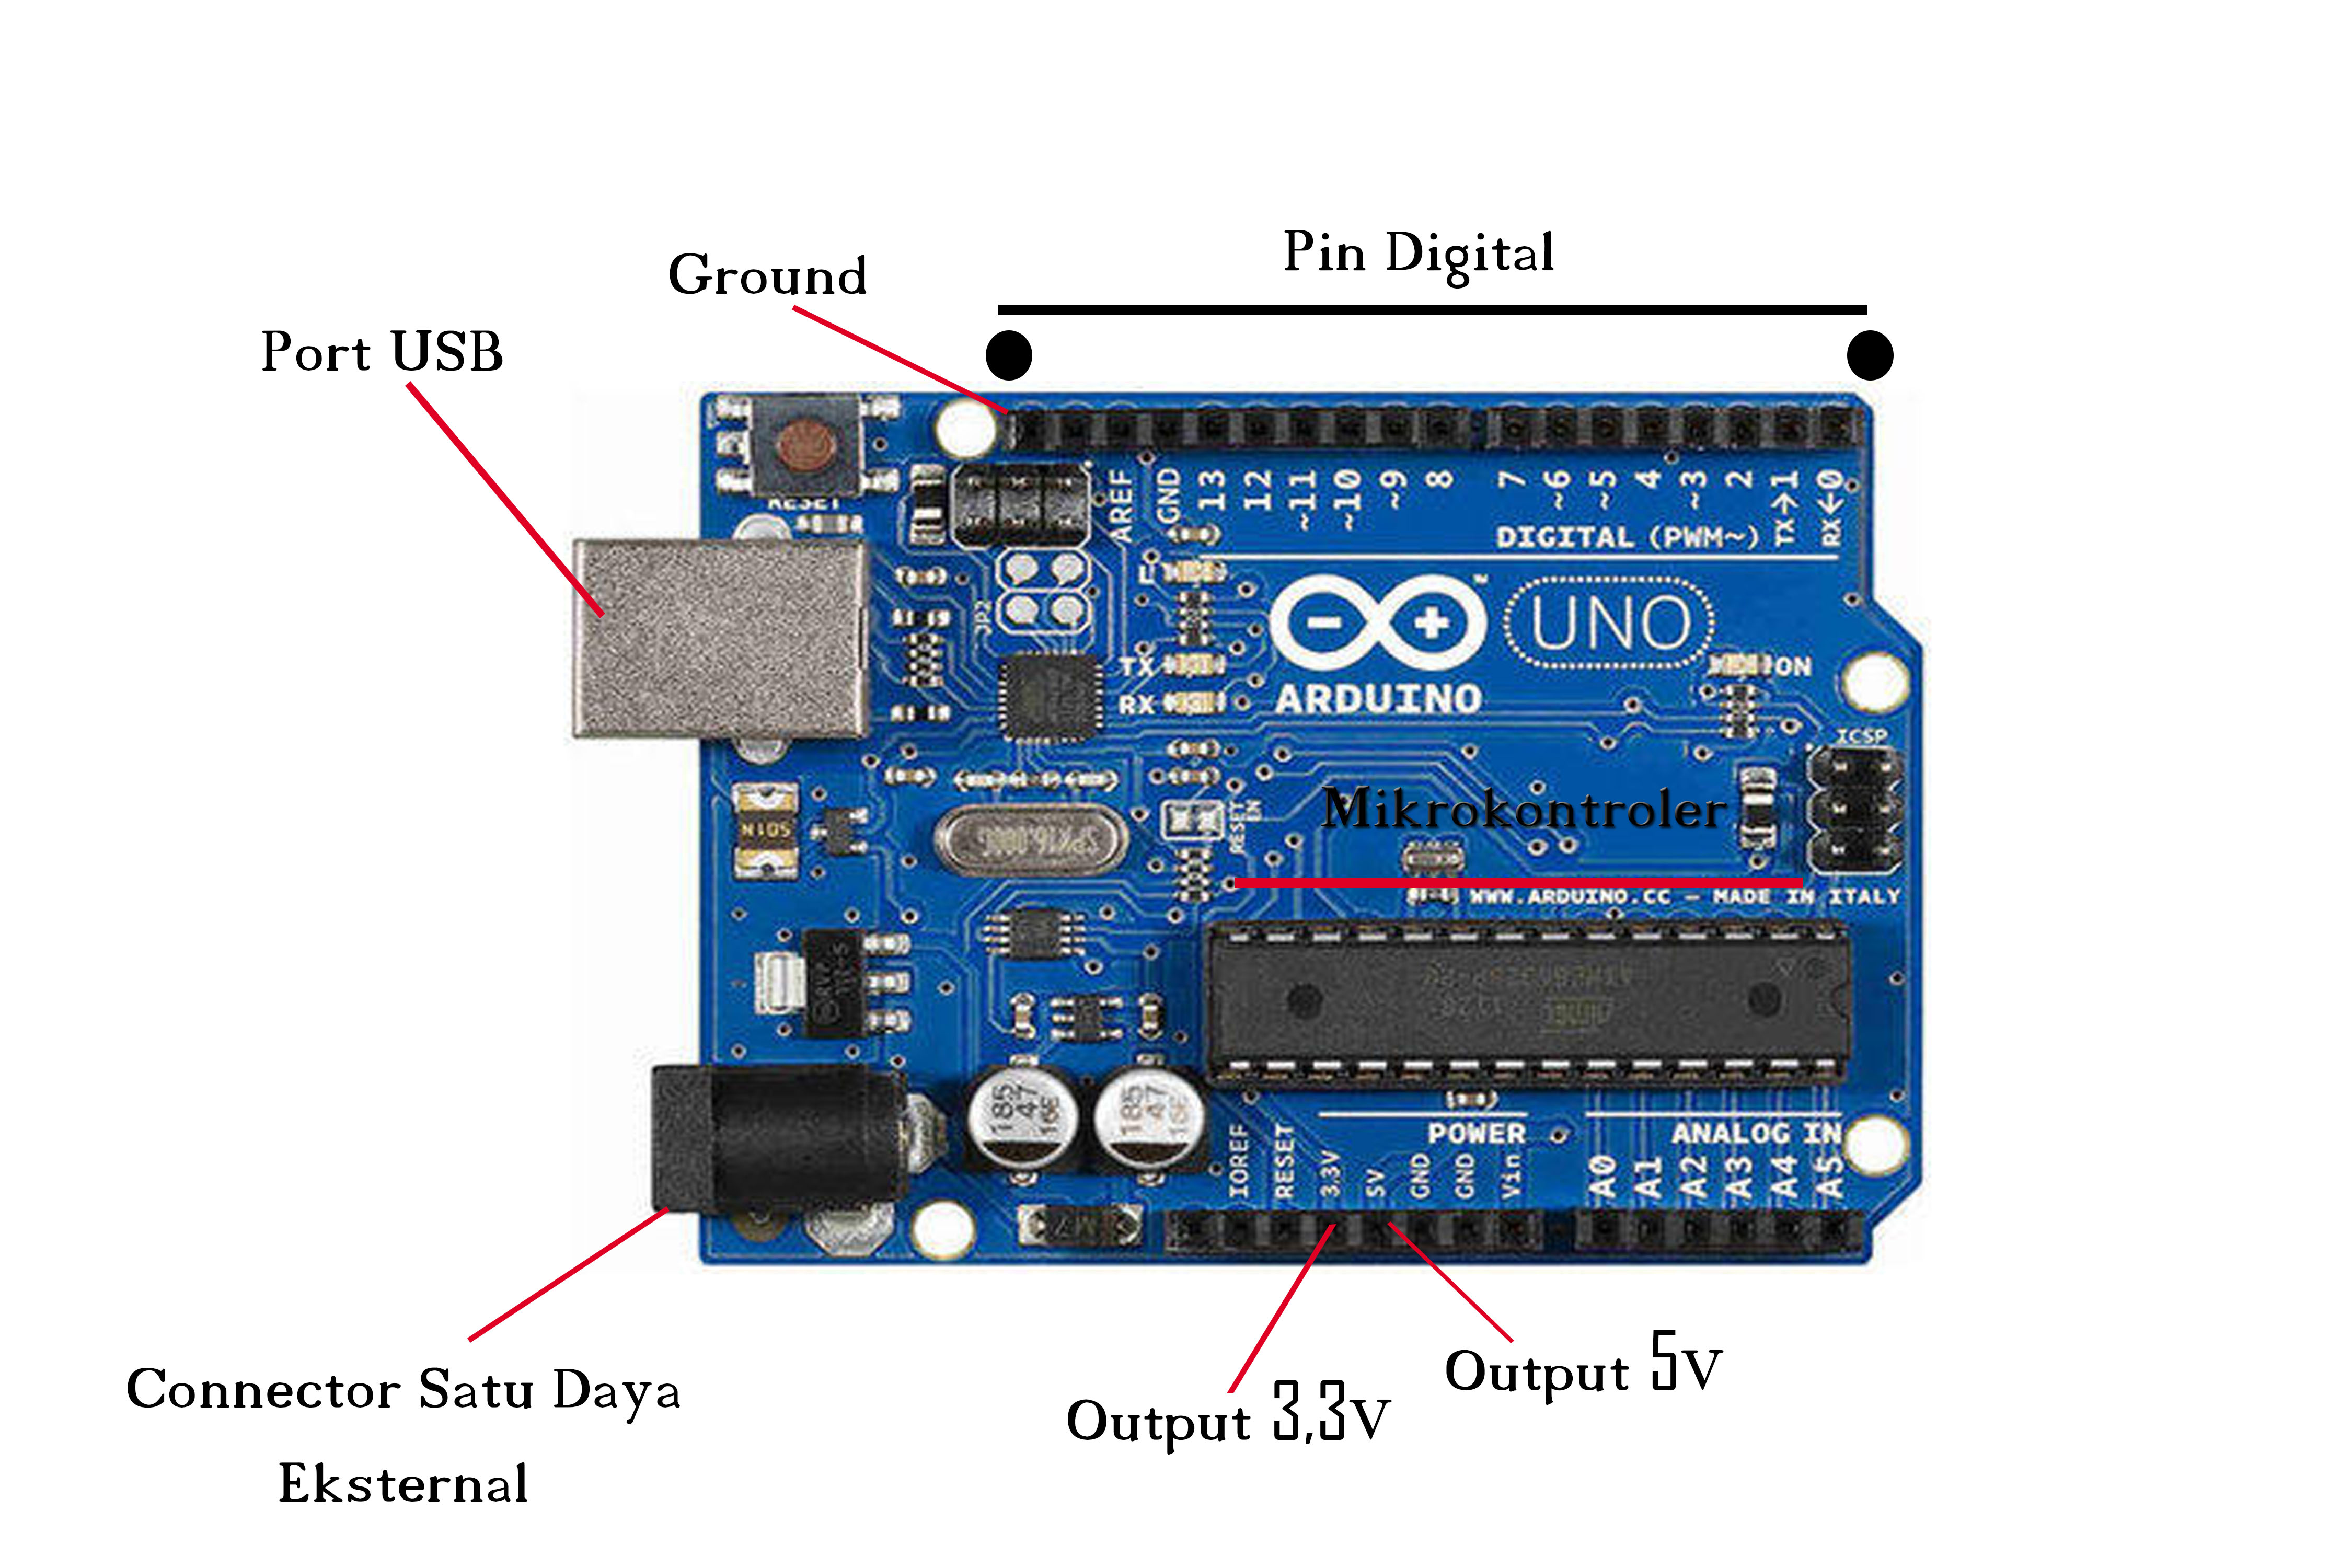
\includegraphics[width=.75\textwidth]{figures/HRD/arduino.jpg}
\caption{Penjelasan Beberapa Bagian Arduino Uno}\label{fig:arduino}
\end{figure}

Pada gambar \ref{fig:ardino} terdapat beberapa bagian pada Arduino Uno. Berikut adalah penjelasan dari masing-masing bagian tersebut :
\begin{itemize}
\item \textbf{Port USB} digunakan untuk menghubungkan Arduino Uno dengan komputer melalui sepasang kabel USB.
\item \textbf{Connector Catu Daya Eksternal} digunakan untuk memasok sumber daya listrik untuk Arduino Uno ketika tidak dihubungkan ke dalam komputer. Jika Arduino Uno terhubung ke komputer melalui USB, maka pasokan daya listrik akan dialirkan melalui komputer menuju Arduino Uno.
\item \textbf{Pin Digital} merupakan pin yang memiliki label 0 sampai dengan 13. Disebut pin digital dikarenakan pin tersebut memiliki isyarat digital berupa 0 atau 1. Dalam pengimplementasiannya, nilai 0 akan dinyatakan dengan tegangan 0 V sementara nilai 1 dinyatakan sebagai tegangan 5 V.    
\item \textbf{Pin Analog} merupakan pin yang bersifat analog atau memiliki nilai yang saling berkesinambungan. Pada program, nilai setiap pin analog yang berlaku sebagai masukan (hasil dari sensor) berkisar antara 0 sampai 1203.
\item \textbf{Atmega328} merupakan mikrokontroler yang digunakan pada Arduino Uno.
\item Terdapat dua pin yang digunakan untuk memasok catu daya ke dalam komponen elektronis yang digunakan dalam menangani suatu project atau experimen, misalnya sensor gerak, sensor jarak dan relai. Tegangan yang tersedia adalah 3,3V dan 5V. Komponen-komponen elektronis yang akan diberikan tegangan oleh Arduino Uno hanyalah komponen yang memerlukan arus kecil.
\end{itemize}   